\section{Background}

\subsection{Maximum Matching Computation using Augmenting Path}
In a general graph $G$, a \emph{matching} $M$ is a set of edges with no shared endpoint.
Edges in $M$ are \emph{matched}; all other edges are \emph{unmatched}.
A vertex is \emph{exposed} if it is incident to no matched edge, and the matching size $|M|$ is the number of matched edges.
In Fig.~\ref{Diagram:MaximumMatching}(a), $M=\{(2,3),(4,5)\}$ has size two, and vertices $1$ and $6$ are exposed.

A matching is \emph{maximum} if no larger matching exists.
Maximum matching algorithms rely on \emph{augmenting paths}: alternating paths whose endpoints are exposed.
Flipping the matched and unmatched edges along such a path replaces a non-maximum matching with a strictly larger one.
In Fig.~\ref{Diagram:MaximumMatching}(a), the path $1\!-\!2\!-\!3\!-\!5\!-\!4\!-\!6$ is augmenting because it alternates between unmatched and matched edges and starts and ends at exposed vertices.
Flipping it yields $M'=\{(1,2),(3,5),(4,6)\}$ in Fig.~\ref{Diagram:MaximumMatching}(b), which is maximum because all vertices are matched.

\begin{figure}[!htbp]
	\centering
	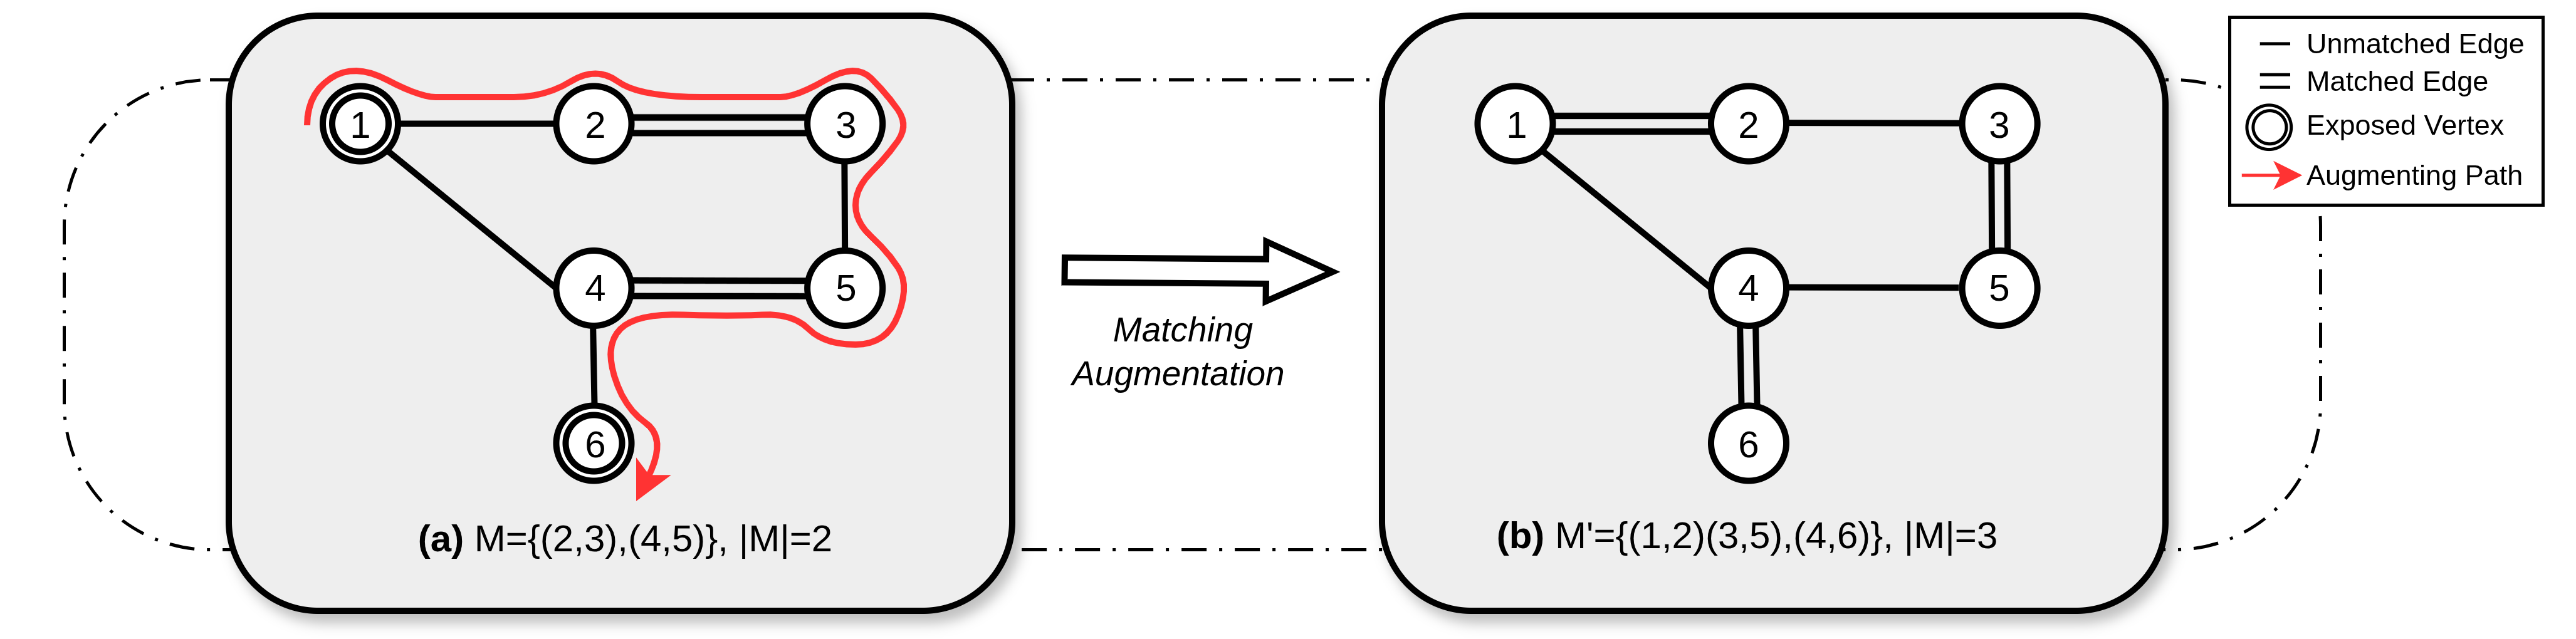
\includegraphics[width=0.80\columnwidth]{figures/diagrams/maximmum_matching.drawio.png}
	\captionsetup{skip=4pt}
	\caption{Maximum Matching and Augmenting Path}
	\label{Diagram:MaximumMatching}
\vspace{-4pt}
\end{figure}

Berge's theorem states that a matching is maximum iff no augmenting path exists.
Thus, Algorithm~\ref{Algo:MaximumMatchingAlgo} starts from the empty matching, repeatedly calls \textsc{Find-Augmenting-Path}, and augments along any returned path until the procedure returns empty.

\begin{algorithm}[!htbp]
  \small
  \captionsetup{font = footnotesize}
  \caption{The Maximum Matching Algorithm}
  \label{Algo:MaximumMatchingAlgo}
  \begin{algorithmic}[1]
    \Require A graph $G$
    \Ensure A maximum matching $M$

    \State $M \gets \emptyset$
    \Repeat
      \State $P \gets$ \Call{Find-Augmenting-Path}{$G$, $M$}
      \If{$P \neq \emptyset$}
        \State $M \gets (M \setminus P) \cup (P \setminus M)$ \Comment{augment $M$ along $P$}
      \EndIf
    \Until{$P = \emptyset$}
    \State \Return $M$

  \end{algorithmic}
\end{algorithm}

\subsection{Augmenting-Path Search via Alternating Trees}
Augmenting-path search uses an \emph{alternating forest}: alternating trees rooted at exposed vertices.
Each node is labeled even or odd by its depth from the root; exposed roots are even.
In Fig.~\ref{Diagram:AlternatingTrees}(a)--(b), exposed nodes~1 and~6 initialize two even-rooted trees.

\begin{figure}[!h]
	\centering
	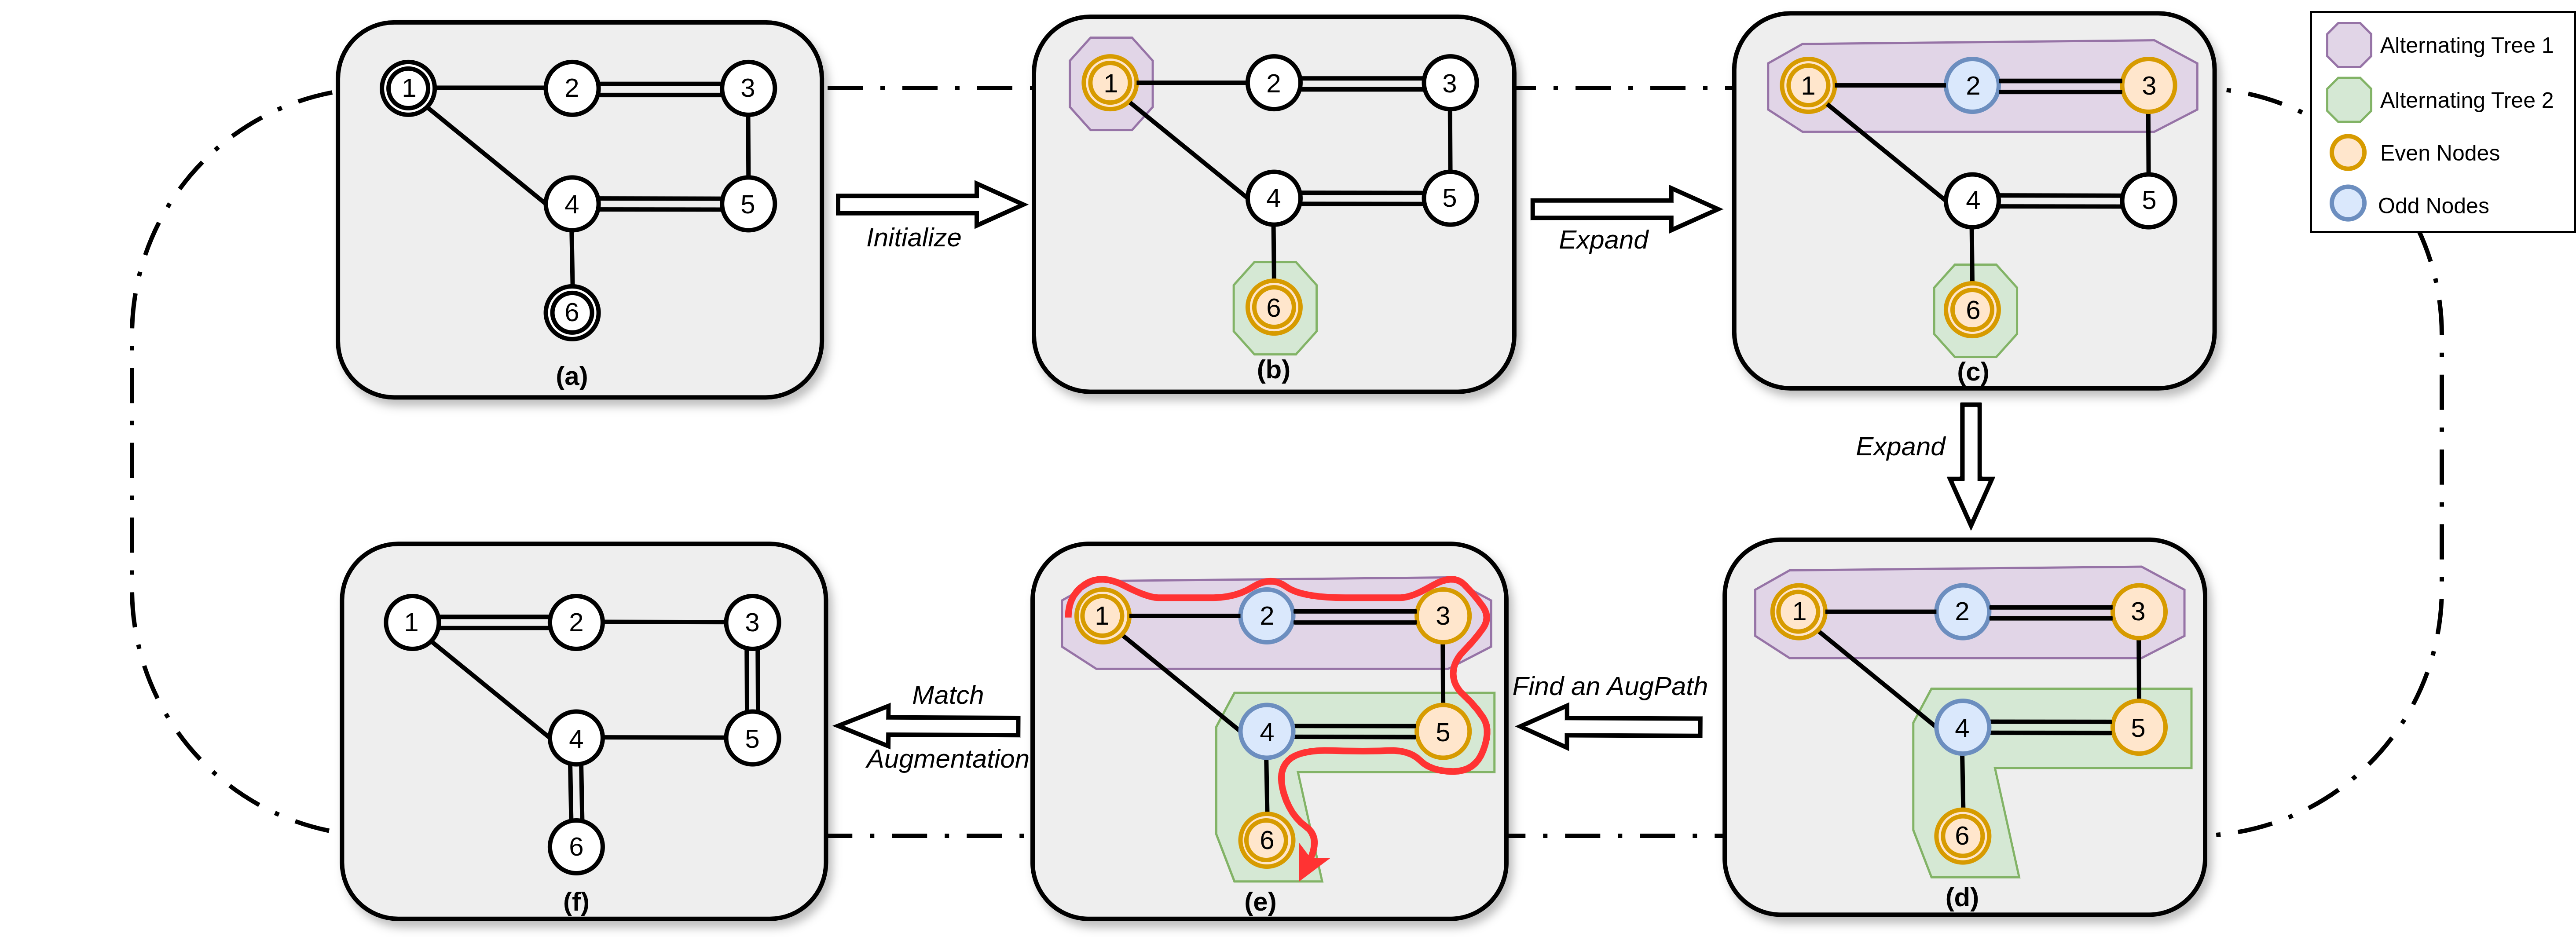
\includegraphics[width=1.0\columnwidth]{figures/diagrams/AlternatingTreesFewerSamples.drawio.png}
	\captionsetup{skip=4pt}
	\caption{The Augmenting-Path Search Procedure using Alternating Trees}
	\label{Diagram:AlternatingTrees}
\vspace{-4pt}
\end{figure}

% Expansion
Expansion starts only from even nodes and proceeds in two-edge steps: an unmatched edge to an odd node, then a matched edge to a new even node.
This preserves the invariant that every root-to-vertex path in an alternating tree has even length and starts with an unmatched edge.
In Fig.~\ref{Diagram:AlternatingTrees}(c), Tree~1 expands from node~1 to node~2 through an unmatched edge and then to node~3 through a matched edge, making nodes~2 and~3 odd and even, respectively.
Similarly, Fig.~\ref{Diagram:AlternatingTrees}(d) expands Tree~2 from node~6 through node~4 to node~5.
If an unmatched edge connects even vertices from different trees, their root-to-vertex paths plus this edge form an augmenting path.
In Fig.~\ref{Diagram:AlternatingTrees}(e), edge $(3,5)$ yields $1\!-\!2\!-\!3\!-\!4\!-\!5\!-\!6$, producing the larger matching in Fig.~\ref{Diagram:AlternatingTrees}(f).


% Key issue with this alternating-tree-expansion and augmenting-path detection mechanism => Blossom

\subsection{The Blossom Anomaly and Two Algorithmic Remedies}
% Although alternating trees work perfectly in bipartite graphs, their expansion may fail to discover an augmenting path in general graphs due to the presence of \emph{blossoms}.  
% A blossom is an odd-length alternating cycle that arises when two even-length root-to-vertex alternating paths in the \textbf{same} alternating tree are connected by an unmatched edge.
% And one node v of the cycle, the base of this blossom is such a node that there exists an alternating path of even length from this node to an exposed vertex.
% For example, in Fig.~\ref{Diagram:Blossoms}(a), the graph forms a blossom $1\!-\!2\!-\!3\!-\!5\!-\!4\!-1$ because the two even-length alternating paths $1\!-\!2\!-\!3$ and $1\!-\!4\!-\!5$ become connected by the unmatched edge $(3,5)$. And 1 is the base of this blossom because it has a even-length path of 0 from it to an exposed node, which is itself.

% Blossoms must be handled carefully because many of the alternating expansion patterns permitted by a blossom fail to expose augmenting paths that actually exist in the graph.  
% For instance, Fig.~\ref{Diagram:MaximumMatching} and ~\ref{Diagram:AlternatingTrees} shows that the graph indeed contains an augmenting path with respect to the given matching.  
% However, the blossom also permits an alternative expansion sequence that conforms to the alternating-tree expansion rules yet still fail to detect any augmenting path, since no unmatched edge ever connects two even vertices from distinct alternating trees.  

% % Two Blossom algorithms
% Blossom algorithms are augmenting-path search procedures with specific blossom handling subroutines.
% To our best knowledge, two sequential blossom algorithms are introduced: the classical recursive blossom algorithm and its modern non-recursive counterpart.
% Both of them handle blossoms by taking into consideration additional alternating-growth patterns necessary for augmenting path detection.
% % Recursive Blossom Algorithm
% The classical recursive algorithm handles a detected blossom by \emph{contracting} the entire odd cycle into a single super-vertex as shown in Fig.~\ref{Diagram:Blossoms}~(e) where the blossom is contracted into a single vertex 7.
% This super-vetex effectively represents all necessary alternating expansions through the contracted blossom.
% After that, in Fig.~\ref{Diagram:Blossoms}~(f) the augmenting-path search will continue on the contracted graph which results in an augmenting path (7,6)
% Then the algorithm performs a \emph{lifting} step in Fig~\ref{Diagram:Blossoms}~(g), expanding each contracted blossom with an even-length path from blossom base 1 to the connect node 4 in reverse order to recover a valid augmenting path in the original graph. 
% % Recursive-Free Blossom Algorithm
% For recursive-free blossom algorithm, upon detecting a blossom, the algorithm instead transform all odd nodes in the blossom into even nodes with a vliad even-length alternating path to the tree root. 
% This "evenification" of the blossom exposes new expansion opportunities, allowing formerly odd vertices to initiate further alternating-tree growth and augmenting-path detection
% In Fig~\ref{Diagram:Blossoms}~(i), nodes 2 and 4 are transformed into even nodes with even-length path 14532 and 12354. 
% After that, the augmenting path can be formed by connecting nodes 4 and 6 since both of them are even nodes.

Alternating-tree expansion is sufficient in bipartite graphs but can fail in general graphs because of \emph{blossoms}.
A blossom is an odd alternating cycle formed when an unmatched edge connects two even vertices in the same alternating tree; its \emph{base} has an even alternating path to an exposed root.
In Fig.~\ref{Diagram:Blossoms}(c), vertices $1\!-\!2\!-\!3\!-\!5\!-\!4\!-1$ form a blossom, and vertex~1 is the base.
Blossoms must be handled carefully because they permit alternating expansion patterns that obey the local tree rules but still fail to expose augmenting paths that exist in the graph.
Without special handling, the valid augmenting path shown in Figs.~\ref{Diagram:MaximumMatching} and~\ref{Diagram:AlternatingTrees} can be missed, as Fig.~\ref{Diagram:Blossoms}(a)--(c) illustrates.

\begin{figure}[!h]
	\centering
	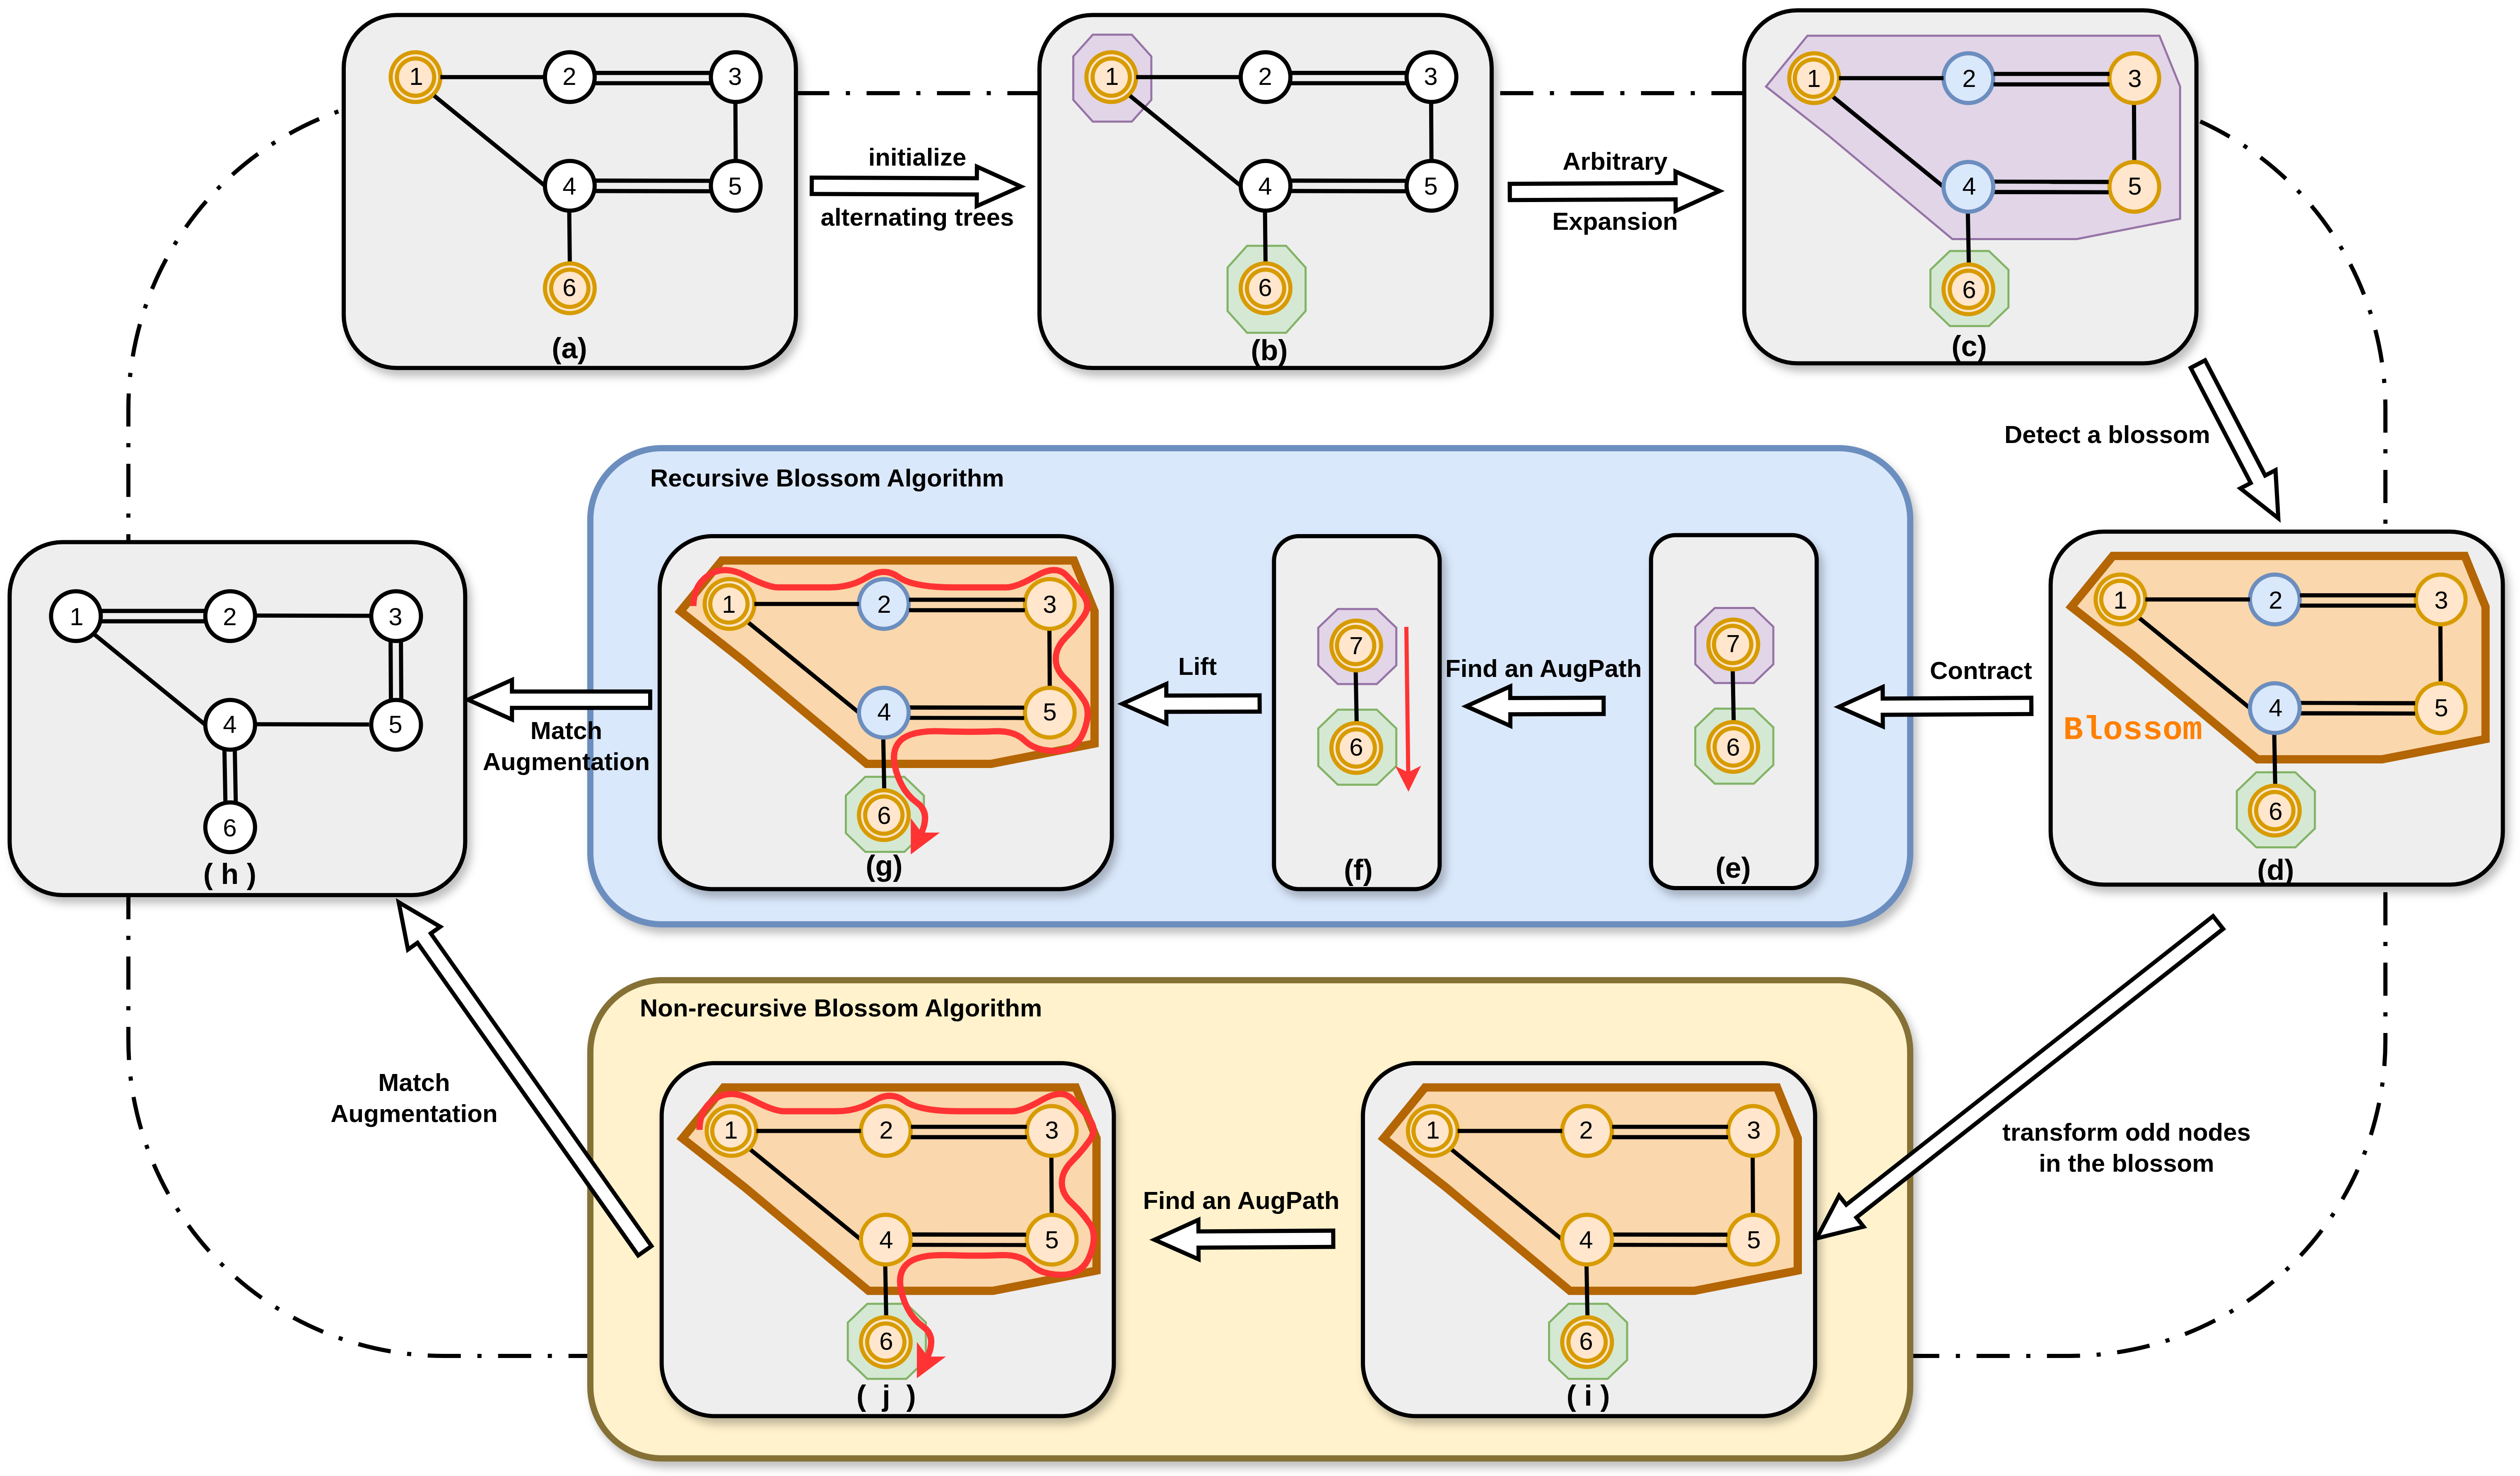
\includegraphics[width=0.95\columnwidth]{figures/diagrams/Blossoms.drawio.png}
	\captionsetup{skip=4pt}
	\caption{The formation of Blossoms and Two Blossom algorithms}
	\label{Diagram:Blossoms}
\vspace{-4pt}
\end{figure}

Two sequential remedies are commonly used: the classical recursive blossom algorithm and a recursion-free variant.
The recursive algorithm contracts a detected blossom into a super-vertex, continues the search on the contracted graph, and then \emph{lifts} the result back to the original graph.
In Fig.~\ref{Diagram:Blossoms}(d)--(h), the blossom becomes vertex~7; after an augmenting path is found, lifting selects the even path $4\!-\!5\!-\!3\!-\!2\!-\!1$ to reconstruct the original augmenting path.

The recursion-free algorithm avoids contraction by converting each odd blossom vertex into an even vertex with a valid even-length alternating path from the root.
This ``evenification'' lets these vertices continue tree expansion.
In Fig.~\ref{Diagram:Blossoms}(i), nodes~2 and~4 become even via paths $1\!-\!4\!-\!5\!-\!3\!-\!2$ and $1\!-\!2\!-\!3\!-\!5\!-\!4$; Fig.~\ref{Diagram:Blossoms}(j) then exposes an augmenting path.


\subsection{X-Blossom Parallel Framework}
The recursion-free algorithm is more amenable to parallelization because it avoids contraction and lifting, whose dynamic graph updates serialize computation.

% X-Blossom
X-Blossom is a parallel framework based on the recursion-free blossom algorithm for parallel augmenting-path search. As shown in Algorithm~\ref{Algo:XBlossom}, it maintains three auxiliary data structures:
\begin{itemize}[leftmargin=*]
    \item The checking set (frontier) $N$, containing the active even vertices whose incident edges are examined in the current iteration.
    \item The alternating forest $F$, consisting of alternating trees rooted at exposed vertices, each representing an independent search structure where even nodes are stored as the search progresses.
    \item The augmenting-path set $P$, which stores augmenting paths discovered during the search.
\end{itemize}

After initializing these structures from the exposed vertices, X-Blossom repeatedly executes three internally parallel procedures in sequence:  
(1) augmenting-path detection,  
(2) alternating-tree expansion, and  
(3) blossom handling.  
The iteration terminates either if an augmenting path is found or if no new even vertices can be generated, indicating that no further augmenting paths exist.
\phantomsection\label{para:xblossom-three-parallel-procedures}
\textcolor{blue}{At the implementation level, all three procedures partition the current checking set across worker threads, and each thread repeatedly scans the incident edges of its assigned frontier vertices.
Procedure~(1) detects augmenting paths by examining unmatched edges between even vertices from different alternating trees and recording vertex-disjoint candidates.
The expansion step then advances the search frontier: Procedure~(2) finds unmatched neighbors outside the current forest, follows their matched partners, and inserts the newly reached even vertices into the next frontier.
For blossom handling, Procedure~(3) inspects edges between even vertices in the same tree, identifies blossom structures, and converts eligible odd vertices into even vertices for subsequent expansion.}

% \vspace{-4pt}
\begin{algorithm}[!htbp]
  % \small
  \footnotesize
  \captionsetup{font = footnotesize}
  \caption{Parallel Augmenting-Path Search Procedure in X-Blossom}
  \label{Algo:XBlossom}
  \begin{algorithmic}[1]

  \Require Graph $G$ and matching $M$
  \Ensure A set of vertex-disjoint augmenting paths $P$, or empty if none exist

  \State $N \gets$ set of exposed vertices
  \State $F \gets$ set of trees rooted at exposed vertices
  \State $P \gets \emptyset$

  \While{$P = \emptyset \wedge N \neq \emptyset$}

      \State $P \gets$ \Call{Parallel-Augmenting-Path-Detection}{$G, M, N, F$}

      \State $N_{\text{next1}} \gets$ \Call{Parallel-Expand-Alternating-Trees}{$G, M, N, F$}

      \State $N_{\text{next2}} \gets$ \Call{Parallel-Blossom-Handling}{$G, M, N, F$}
      
      \State $N \gets N_{\text{next1}} \cup N_{\text{next2}}$

  \EndWhile
  
  \State \Return $P$

  \end{algorithmic}
\end{algorithm}
\vspace{-4pt}
